\section{正数和负数}

\begin{frame}\frametitle{为什么会存在负数?}\pause
	\begin{block}{1、日常生活需要}\pause
		\begin{itemize}
			\item 建国以后北京历史最低温度:零下 \SI{27.4}{\degreeCelsius}(1966) \quad\pause \underline{\SI{-27.4}{\degreeCelsius}}\pause
			\item 中国大陆最低点(新疆吐鲁番艾丁湖洼地)海拔:海平面以下$154.31$米 \quad\pause \underline{$-154.31\text{m}$}\pause
			\item 2018年5月9日上证指数:下跌$2.35$个点,收于3159.15个点\quad\pause \underline{\color{fall-green}$-2.35$}\pause
			\item 支出,负资产……
		\end{itemize}
	\end{block}	
\end{frame}

\begin{frame}\frametitle{为什么会存在负数?}
	\begin{block}{2、数学的对称性}\pause
		正整数具有如下运算规律:
		\begin{enumerate}
			\item 加法交换律:$a + b = b + a$
			\item 加法结合律:$(a + b) + c = a + (b + c)$
			\item 乘法交换律:$a \times b = b \times a$
			\item 乘法分配率:$a \times (b + c) = a \times b + a \times c$
			\item 加法单位元:$a + 0 = 0 + a = 0$
			\item 乘法零元:$a \times 0 = 0 \times a = 0$
		\end{enumerate}
	\end{block}	\pause
	\begin{question}
		什么数满足:$\boxed{?} + 1 = 0$
	\end{question}
\end{frame}

\begin{frame}\frametitle{为什么会存在负数?}
	解方程:
	\[\begin{WithArrows}
		x + 1 &= 0 \\ \pause
		x &= 0 - 1 \pause \Arrow{省去 $0$} \\
		x &= -1
	\end{WithArrows}\] \pause
	\begin{definition}{\alert{负整数}}
		设 $a$ 为整数,则
		\[-a = 0 - a\]
	\end{definition}\pause
	\vspace{1ex}
	对于负分数,我们可以作同样的定义。
\end{frame}

\begin{frame}{负数的运算法则}\pause
	\begin{block}{加减法}\pause
		\begin{enumerate}[<+- | alert@+>]
			\item $a + (-b) = a + (0-b) = (a + 0) - b = a - b$
			\item $-a + b = (-a) + b = b + (-a) = b - a$
			\item $ -a + (-b) = (-a) + (-b) = (-a) - b = 0 - a - b = 0 - (a + b) = -(a + b)$
			\item $a - (-b) = a - (0 - b) = a - 0 + b = a + b$
			\item $-a - (-b) = -a + b = b - a$
		\end{enumerate}
	\end{block}
	\begin{alertblock}<8>{规律}
		\qquad 负号$\approx$减号
	\end{alertblock}
\end{frame}

\begin{frame}{负数的运算法则}
	\begin{center}
		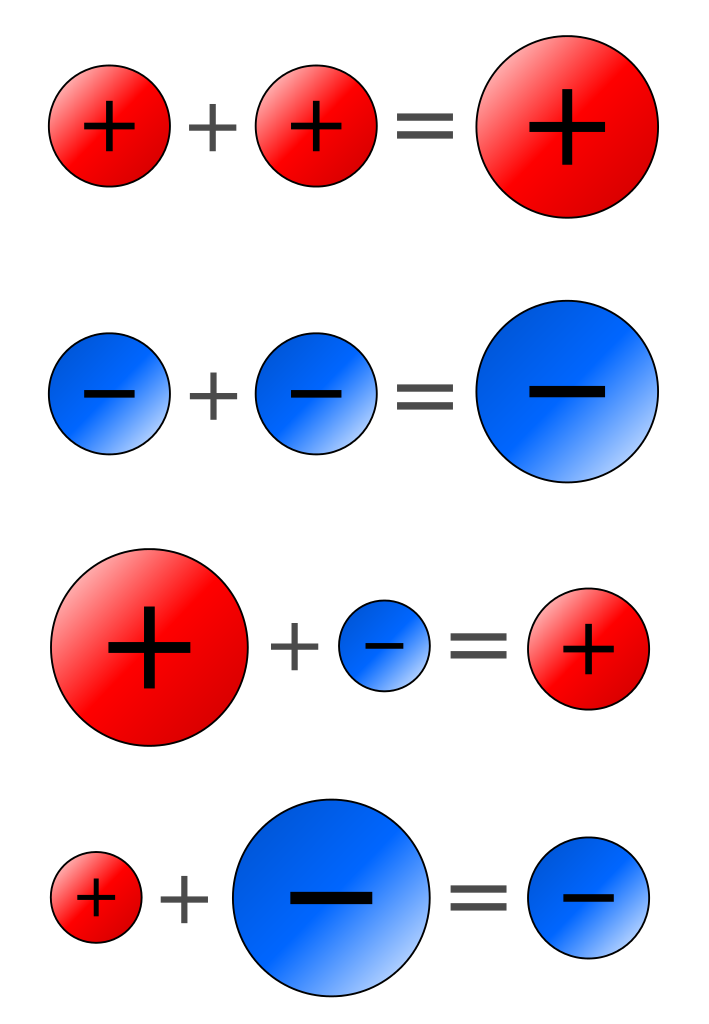
\includegraphics[height=0.8\textheight]{AdditionRules.png}
	\end{center}
\end{frame}

\begin{frame}{负数的运算法则}
	\begin{block}{乘法} \pause
		\begin{enumerate}[<+- | alert@+>]
			\item $a \times (-b) = a \times (0 - b) = a \times 0 - a \times b = 0 - a \times b = - a \times b$
			\item $(-a) \times b = b \times (-a) = - b \times a = - a \times b$
			\item $(-a) \times (-b) = - a \times (-b) = - (- a \times b) = a \times b$
			\item $(-a) \div b = - a \div b$
			\item $a \div (-b) = - a \div b$
			\item $(-a) \div (-b) = a \div b$
		\end{enumerate}
	\end{block}
	\begin{alertblock}<8>{规律}
		\qquad 负负得正,奇负偶正
	\end{alertblock}
\end{frame}

\begin{frame}
	\begin{alertblock}{注意}
		正负是相对的!
	\end{alertblock}
\end{frame}